\documentclass[compress,professionalfont]{beamer}
\mode<presentation>
\setbeamertemplate{navigation symbols}{}
\usetheme{Madrid}

% pdf is displayed in full screen mode automatically
\hypersetup{pdfpagemode=FullScreen}

\usepackage[utf8]{inputenc}
\usepackage[T2A]{fontenc}
\usepackage[russian]{babel}

\usepackage{graphics, graphicx}
\usepackage{amsmath}
\usepackage{amssymb}
\usepackage{amsfonts}
\usepackage{tikz,pgfplots}
\usepackage{pgfplots, epstopdf}
\usepackage{subfigure}
\usepackage{cmap}
%\usepackage{helvet}
\usebeamerfont{Times}
\usepackage{ragged2e}

\definecolor{darkred}{RGB}{16,78,139}
\newcommand{\myStandartColoredItem}[1]{{\color{darkred}\bf{{#1}}}}

\makeatletter
\long\def\beamer@author[#1]#2{%
	\def\insertauthor{\def\inst{\beamer@insttitle}\def\and{\beamer@andtitle}%
		\begin{tabular}{ll}#2\end{tabular}}%
	\def\beamer@shortauthor{#1}%
	\ifbeamer@autopdfinfo%
	\def\beamer@andstripped{}%
	\beamer@stripands#1 \and\relax
	{\let\inst=\@gobble\let\thanks=\@gobble\def\and{, }\hypersetup{pdfauthor={\beamer@andstripped}}}
	\fi%
}
\makeatother

\titlegraphic{
\includegraphics[width=2.cm]{emblema.eps}}
\title[]{ПРИМЕНЕНИЕ МЕТОДОВ МАШИННОГО ОБУЧЕНИЯ ДЛЯ РЕШЕНИЯ ЗАДАЧИ ФИЛЬТРАЦИИ НЕЖЕЛАТЕЛЬНЫХ ДАННЫХ}
\author[Разумов Т.Е.]{
Выполнил студент группы ФН1-41М& Разумов~Т.Е. \\
Научный руководитель, д.ф.--м.н., проф.& Кравченко~В.Ф. \\
Научный консультант, ст.преп.& Кравченко~О.В. 
}
\institute[]{МГТУ им. Н.Э.~Баумана}
\date{21 июня 2021 г.}

\graphicspath{{images/}}


\begin{document}

%\justify

%%%%%%%%%%%%%%%%%%%%%%%%%%%%%%%%%%%%%%
\begin{frame}[plain]
	\maketitle
\end{frame}

%%%%%%%%%%%%%%%%%%%%%%%%%%%%%%%%%%%%%%
\begin{frame}
\frametitle{Актуальность проблемы}

\begin{center}
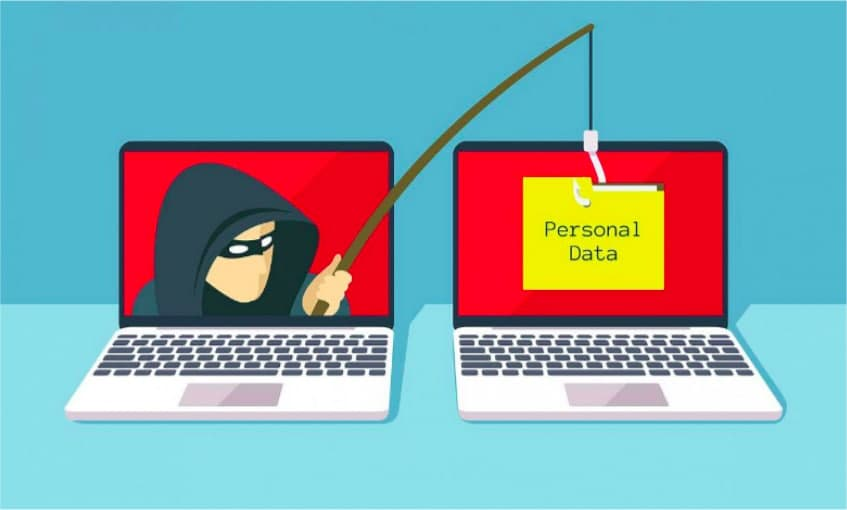
\includegraphics[width=0.45\textwidth]{actual1.jpg}
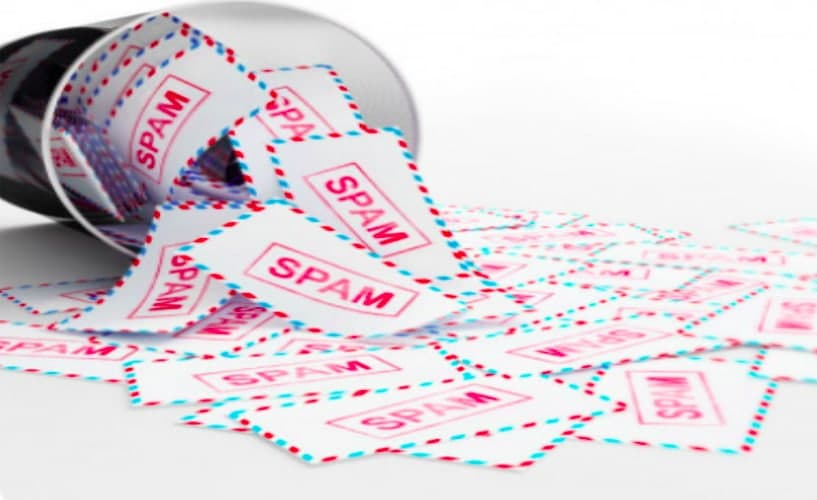
\includegraphics[width=0.45\textwidth]{actual2.jpg}
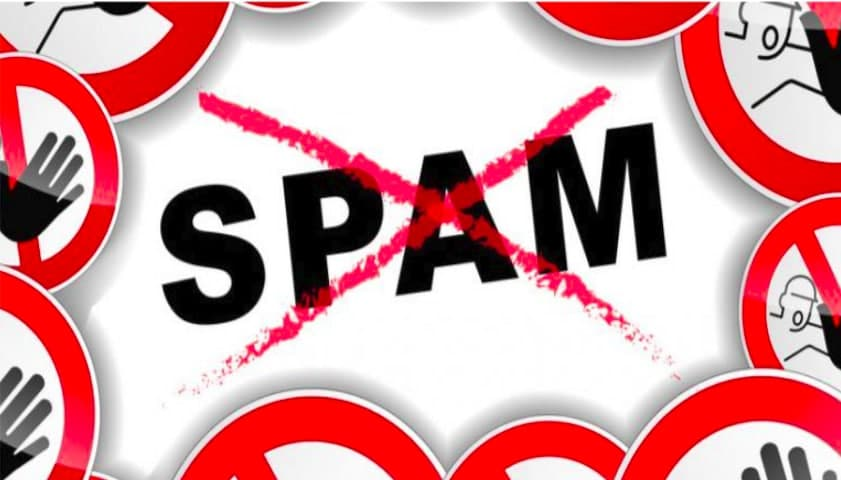
\includegraphics[width=0.45\textwidth]{actual3.jpg}

\includegraphics[width=0.45\textwidth]{actual4.jpg}
\end{center}
\end{frame}

%%%%%%%%%%%%%%%%%%%%%%%%%%%%%%%%%%%%%%
\begin{frame}
\frametitle{Постановка задачи}

В рамках работы требуется реализовать \emph{спам--фильтр систему} для следующих продуктов Mail.Ru Group: почта, юла, мой мир, ответы, icq, пульс, агент. Ключевыми требованиями на систему являются:
\begin{itemize}
\item Высокая точность --- должно верно классифицироваться не менее 99\% писем.
\item Высокая отказоустойчивость --- сервис, осуществляющий запуск спам--фильтра, должен отвечать не менее чем на 99.99\% запросов.
\item Высокая производительность --- полный цикл проверки письма не должен быть дольше 3--х секунд.
\end{itemize}

Формально постановку задачи можно разбить на 4 этапа:
\begin{enumerate}
\item Предобработка письма.
\item Построение отображения текстовой информации в векторное пространство (векторизация).
\item Классификация объектов.
\item Разработка приложения, имеющего микросервисную архитектуру, для запуска системы на реальных пользователях.
\end{enumerate}

\end{frame}

%%%%%%%%%%%%%%%%%%%%%%%%%%%%%%%%%%%%%%
\begin{frame}

\begin{center}
\Huge\bf Предобработка
\end{center}

\end{frame}

%%%%%%%%%%%%%%%%%%%%%%%%%%%%%%%%%%%%%%
\begin{frame}
\frametitle{Письмо в веб--интерфейсе}

\begin{center}
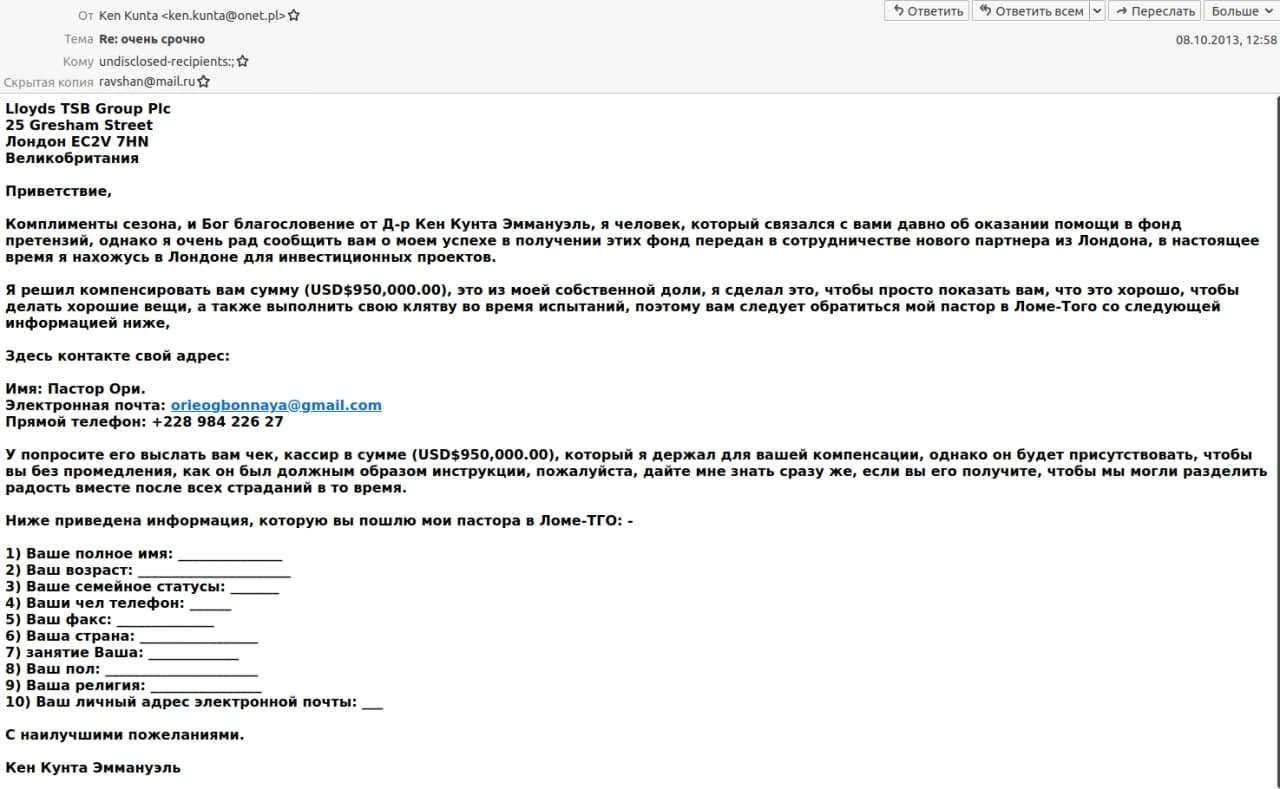
\includegraphics[width=.95\textwidth]{eml.jpg}
\end{center}

\end{frame}

%%%%%%%%%%%%%%%%%%%%%%%%%%%%%%%%%%%%%%
\begin{frame}
\frametitle{Формат исходного сообщения}

\begin{center}
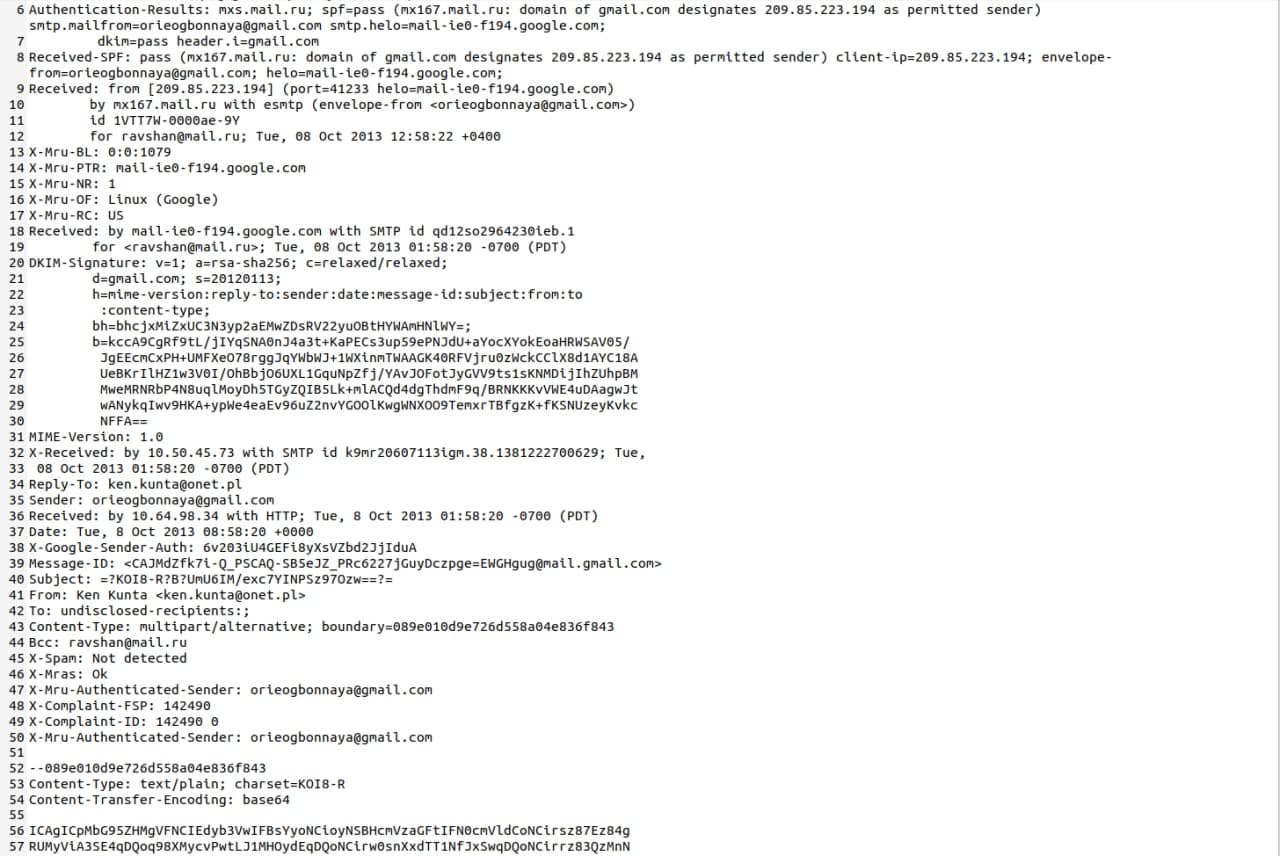
\includegraphics[width=.95\textwidth]{eml_raw.jpg}
\end{center}

\end{frame}

%%%%%%%%%%%%%%%%%%%%%%%%%%%%%%%%%%%%%%
\begin{frame}[fragile=singleslide]
\frametitle{Предобработка}

\textbf{Текстовая информация}
Для извлечения информации из документов, имеющих текстовый формат, таких как docx, html, calendar и.т.д. реализованы собственные специализированные парсеры написанные на \verb|C++| и \verb|Golang|.
\vspace{.5cm}

\textbf{Графическая информация}
Поскольку изображения и pdf не являются текстовыми форматами, то
для автоматического извлечения текста разработано два алгоритма машинного обучения на языке \verb|Python|
\begin{itemize}
\item Модель сегментации и зондирования.
\item Модель извлечения текста.
\end{itemize}

\end{frame}

%%%%%%%%%%%%%%%%%%%%%%%%%%%%%%%%%%%%%%
\begin{frame}
\frametitle{Предобработка}

После извлечения информации из всех вложений письма текст проходит через следующие этапы:
\begin{itemize}
\item Конкатенация всех частей с заданными разделителями.
\item Декодирование в заданную кодировку (utf8, cp1251) и приведение к одному регистру.
\item Удаление лишних пробелов, отступов и стоп--слов.
\item Нормализация:
\begin{enumerate}
\item Стемминг (``кошек'' $\rightarrow$ ``кош'').
\item Лемматизация (``кошек'' $\rightarrow$ ``кошка'').
\end{enumerate}
\end{itemize}

\end{frame}

%%%%%%%%%%%%%%%%%%%%%%%%%%%%%%%%%%%%%%
\begin{frame}

\begin{center}
\Huge\bf Векторизация
\end{center}

\end{frame}

%%%%%%%%%%%%%%%%%%%%%%%%%%%%%%%%%%%%%%
\begin{frame}
\frametitle{Постановка задачи}

Пуcть дано множество всех слов или словосочетаний $W$.

В функциональном анализе доказывается гиперконтинуальность этого множества, что делает невозможным применение численных алгоритмов.

Требуется аппроксимировать данные линейными многообразиями меньшей размерности $W \rightarrow X = \mathbb{R}^n.$

\end{frame}

%%%%%%%%%%%%%%%%%%%%%%%%%%%%%%%%%%%%%%
\begin{frame}
\frametitle{Мешок слов (bow)}

Каждому слову или словосочетанию (терму) ставится в соответствие некоторое число. В этом случае текст определяется вектором $\vec{u} = (u_1, ..., u_N)^T$,
где $N$ --- размерность из конечного словаря $X^l$ состоящего из уникальных термов обучающей выборки. \\
$u_i$ определяется как Булевский вес
$$
u_i = \begin{cases}
1, & \mbox{если элемент присутствует в письме}, \\
0, & \mbox{если элемент не присутствует в письме}.
\end{cases}
$$

\begin{center}
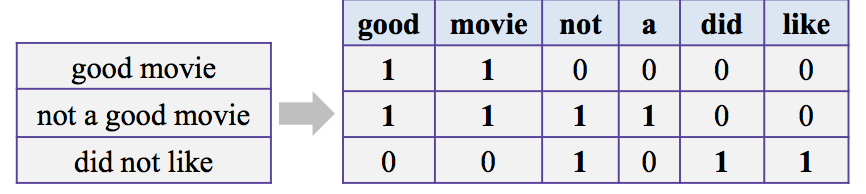
\includegraphics[width=0.6\textwidth]{bow.png}
\end{center}

Основной проблемой bow -- векторизации является потеря контекстной связи между словами и чрезмерно большое потребление памяти.

\end{frame}

%%%%%%%%%%%%%%%%%%%%%%%%%%%%%%%%%%%%%%
\begin{frame}
\frametitle{word2vec}

Учитывая последовательность обучающих слов $w_1, w_2, w_3, ..., w_N$, требуется максимизировать среднюю логарифмическую вероятность
$$
\dfrac{1}{N}\sum_{i=1}^{N}\sum_{-c \leqslant j \leqslant c, j \neq 0} \ln p(w_{i+j}|w_i) \rightarrow \max,
$$
где $c$ --- размер обучающего контекста для слова $w_i$. Вероятность $p(w_O|w_I)$ нахождения слова $w_O$ в контексте со словом $w_I$ определяется через фукцию softmax
$$
p(w_O|w_I) = \dfrac{\exp({\vec{u}_{w_O}\cdot\vec{v}_{w_I}})}{\sum_{i=1}^{N} \exp({\vec{u}_{i} \cdot \vec{v}_{w_I}})},
$$
где $\vec{v}_{w_I}$ --- некий контекстный вектор для слова $w_I$, $\vec{u}_{w_O}$ --- word2vec представление слова $w_O$.
При этом, стоимость вычисления функции softmax пропорциональна $O(N)$, которое на практике является очень большим ($\sim10^9\div10^{12}$).

%\begin{center}
%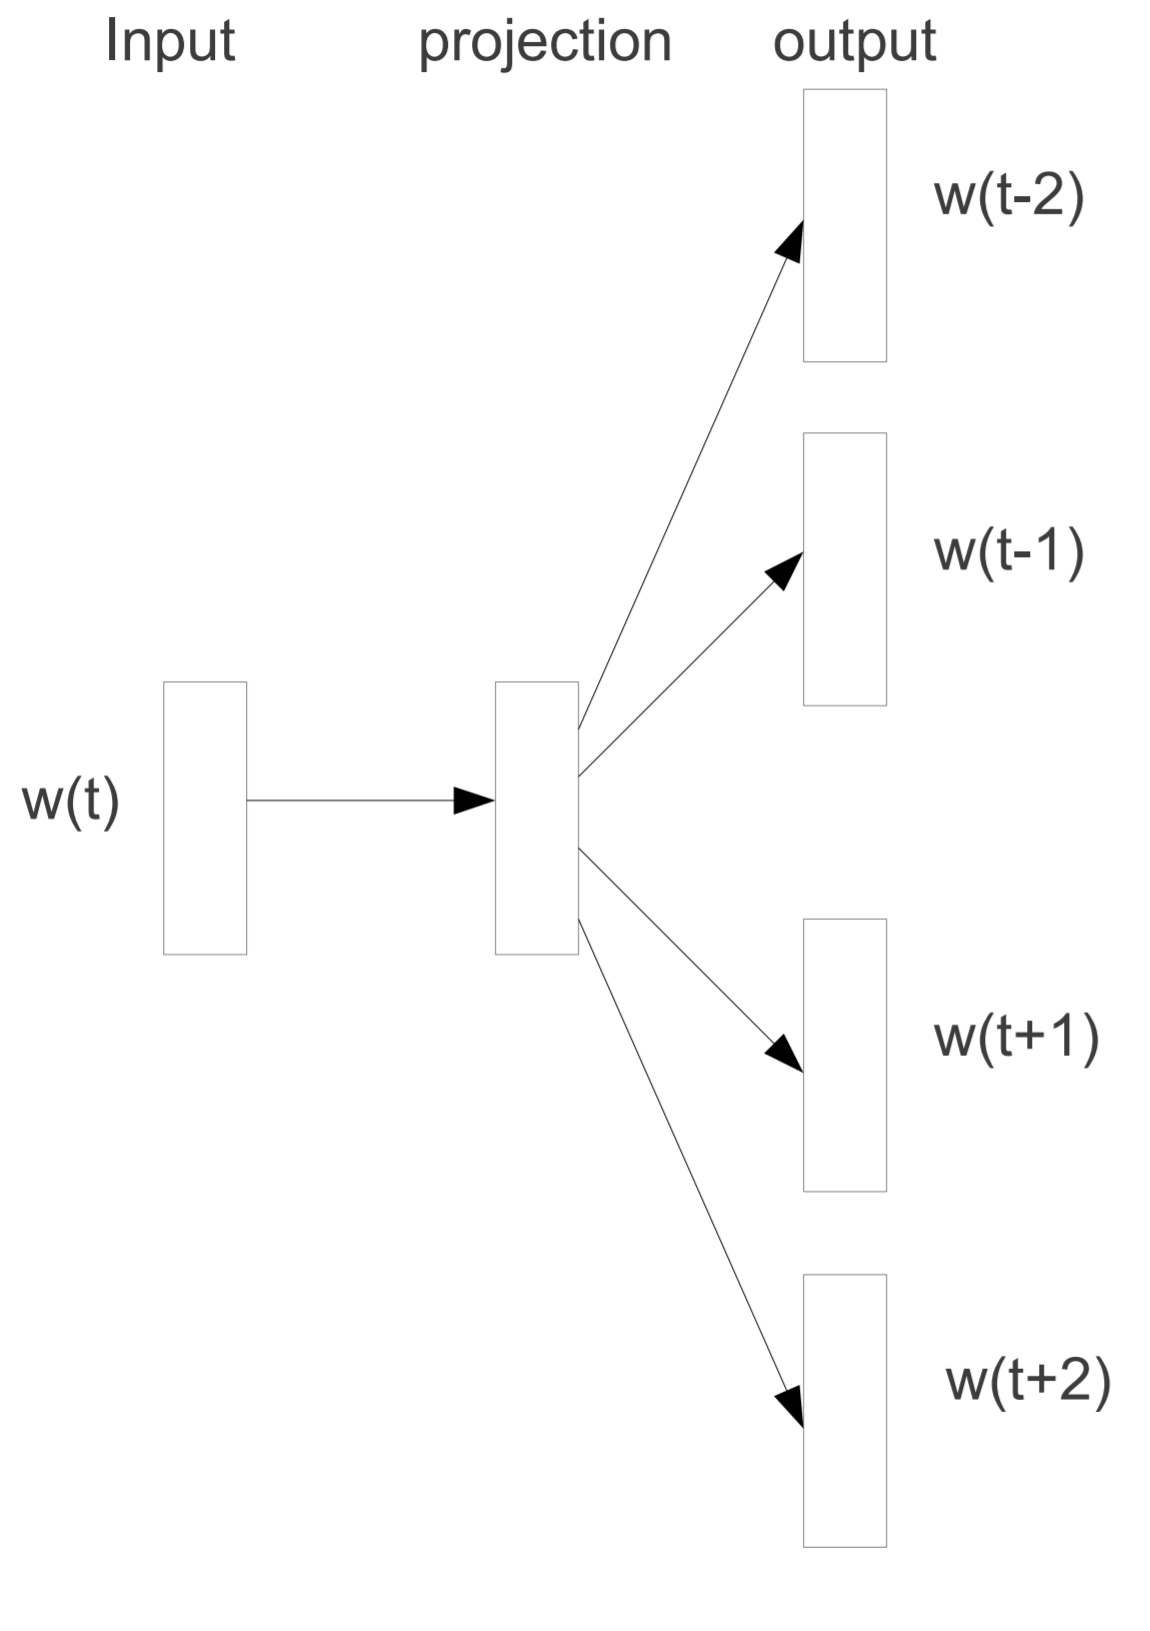
\includegraphics[width=0.25\textwidth]{skip_gram.png}
%\end{center}

\end{frame}

%%%%%%%%%%%%%%%%%%%%%%%%%%%%%%%%%%%%%%
\begin{frame}
\frametitle{Оптимизация word2vec}

Оптимизации заключается в том, что на основе словаря текста строится двоичное дерево Хаффмана
\begin{center}
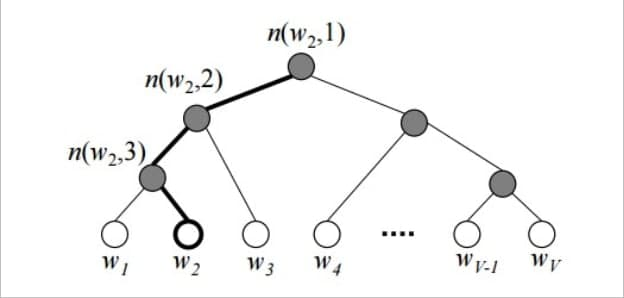
\includegraphics[width=0.35\textwidth]{huffman.jpg}
\end{center}

Тогда выражение для вычисления вероятности $p(w_O|w_I)$ нахождения слова $w_O$ в контексте с $w_I$ имеет вид
$$
p(w_O|w_I) = \prod\limits_{j=1}^{L(w)-1} \sigma \Big(\delta_{n(w,j+1), n_l(w,j)} \vec{u}_{n(w,j)} \cdot \vec{v}_{w_I} \Big),
$$
где $L(w)$ --- расстояние от вершины до слова $w$, $n(w, j)$ --- узел дерева под номером $j$ на пути от вершины до слова $w$, $n_l(w,j)$ --- левый потомок для узла $n(w,j)$, $\sigma(x) = 1 / (1 + e^{-x})$, $\delta_{i,j}$ --- символ Кронекера.

Стоимость вычисления $O(\log_2 N)$.

\end{frame}

%%%%%%%%%%%%%%%%%%%%%%%%%%%%%%%%%%%%%%
\begin{frame}

\begin{center}
\Huge\bf Классификация
\end{center}

\end{frame}

%%%%%%%%%%%%%%%%%%%%%%%%%%%%%%%%%%%%%%
\begin{frame}
\frametitle{Постановка задачи}

Требуется построить отображение из $\mu^{*} : X =  \mathbb{R}^n \rightarrow Y = \{-1,+1\}$ по обучающей выборке $X^l = (\vec{x}_i, y_i)_{i=1}^l$, таким образом, что

$$
\mu^{*}\left(X^l\right) = \operatorname*{argmin}_{\mu \in A}  Q\left(\mu, X^l\right), \quad Q\left(\mu, X^l\right) = \dfrac{1}{l} \sum_{i=1}^{l} Z(\mu, \vec{x}_i, y_i).
$$
где $X$ --- признаковое пространство векторизованных текстов, \\
$\mu$ --- решающая функция, $A$ --- множество решающих функций, \\
$Z$ --- функция потерь, характеризующая величину ошибки функции $\mu$ на объекте $\vec{x}$, $Q$ --- функция эмперического риска, \\
$Y$ --- множество допустимых ответов, \\
Для нашего случая $-1$ --- спам, $+1$ --- не спам. \\

\end{frame}

%%%%%%%%%%%%%%%%%%%%%%%%%%%%%%%%%%%%%%
\begin{frame}
\frametitle{Вероятностная постановка задачи}

Минимизация функции эмпирического риска эквивалетна задаче максимизации функции правдоподобия
$$
L(\vec{\theta}, X^l) = \prod\limits_{i=1}^l f(\vec{x}_i, y_i, \vec{\theta}) \rightarrow \max_{\vec{\theta}},
$$
$$
\ln L(\vec{\theta}, X^l) = \sum_{i=1}^{l} \ln f(\vec{x}_i, y_i, \vec{\theta}) \rightarrow \max_{\vec{\theta}},
$$
где $L$ --- функция правдоподобия, $X^l$ --- обучающая выборка, \\
$f(\vec{x}, y)$ --- совместная плотность распределения случайных величин $\vec{x}$~и~$y$,
$\vec{\theta}$ --- параметры решающей функции.

\end{frame}

%%%%%%%%%%%%%%%%%%%%%%%%%%%%%%%%%%%%%%
\begin{frame}
\frametitle{Логистическая регрессия}
\small

Считаем, что апостериорная вероятность принадлежности произвольного объекта из множества $\vec{x} \in X$ классу $y \in \{-1, +1\}$ может быть вычислена по значению дискриминантной функции
$$
p(y|\vec{x}) = \sigma ((\vec{w} \cdot \vec{x}) y), \quad \sigma(z) = \dfrac{1}{1+ e^{-z}}.
$$

Согласно формуле условной вероятности $p(\vec{x},y) = p(y|\vec{x})p(\vec{x})$, где плотности распределения объектов $\vec{x}$ не зависят от параметров $\vec{w}$, функция максимального правдоподобия примет вид

$$
L\left(\vec{w}, X^l\right) =  \sum_{i=1}^{n} \ln \sigma((\vec{w} \cdot \vec{x})y) + c \rightarrow \max_{\vec{w}}.
$$
Что эквивалентно минимизации функции эмпирического риска
$$
Q\left(\vec{w}, X^l\right) = \sum_{i=1}^{n} \ln{\left(1 + \exp{(-(\vec{w} \cdot \vec{x_i})y_i)}\right)} \rightarrow \min_{\vec{w}}.
$$

Градиентный шаг при настройке параметров $\vec{w}$ с темпом обучения $\eta$
$$
\vec{w} := \vec{w} + \eta\,y_i \vec{x_i} \sigma(-(\vec{w} \cdot \vec{x_i})y_i).
$$

\end{frame}

%%%%%%%%%%%%%%%%%%%%%%%%%%%%%%%%%%%%%%
\begin{frame}[fragile=singleslide]
\frametitle{Полносвязная нейронная сеть (FCNN)}
\small

Полносвязная нейронная сеть для нашей задачи имеет 3 слоя. На каждом слое производится регуляризация данных.
%\begin{center}
%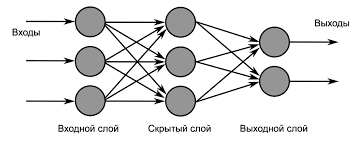
\includegraphics[width=0.55\textwidth]{fcnn.png}
%\end{center}
%
Для решаемой задачи нейронная сеть представляет собой аппроксимационную функцию вида
\begin{align*}
& \mu(x) = h_2 \left(\sum_{k=0}^{n_2} w''_k h_1\left(\sum_{j=0}^{n_1} w'_j h_0\left( \sum_{i=0}^{n_0} w_i x_i \right)\right)\right), \\
& h_2(x) = \dfrac{1}{1+e^{-x}}, \quad h_0(x) = h_1(x) = 
\begin{cases} 
x, & x > 0, \\
0, & x \leqslant 0.
\end{cases}
\end{align*}
где $h_i$ --- функция активации для соответствующего слоя. Для нахождения весовых коэффициентов $\{w_i\}_{i=0}^{n_0}$, $\{w'_j\}_{j=0}^{n_1}$, $\{w''_k\}_{k=0}^{n_2}$ используется метод адаптивной оценки моментов (Adaptive Moment Estimation, Adam) с функцей эмпирического риска
$$
Q\left(\vec{w}, X^l\right) = - \sum_{i=1}^{n} \vec{w} \cdot (y_i \ln \vec{x}_i + (1 - y_i)\ln (1 - \vec{x}_i)).
$$

\end{frame}

%%%%%%%%%%%%%%%%%%%%%%%%%%%%%%%%%%%%%%
\begin{frame}
\frametitle{Сравнение моделей}

$$
\text{precision} = \dfrac{TP}{TP + FP}, \quad \text{accuracy}= \dfrac{TP+TN}{TP+TN+FP+FN},
$$

$$
\text{recall} = \dfrac{TP}{TP + FN}, \quad f_{\beta} = \dfrac{(1 + \beta^2) \cdot \text{precision} \cdot \text{recall}}{\beta^2 \cdot \text{precision} + \text{recall}}.
$$

\begin{center}
\textbf{Логистическая регрессия}

  \begin{tabular}{ | c | c | c | c | c |}
    \hline
               & precision & recall & accuracy & $f_1$ \\ \hline
     bow       & 0.91143 & 0.99961 & 0.91234 & 0.92325 \\ \hline
     word2vec & 0.95523 & 0.89164 & 0.96254 & 0.93645 \\ \hline
  \end{tabular}

\vspace{.5cm}

\textbf{Полносвязная нейронная сеть}
  \begin{tabular}{ | c | c | c | c | c |}
    \hline
               & precision & recall & accuracy & $f_1$ \\ \hline
     bow       & 0.93604 & 0.95643 & 0.97234 & 0.99474 \\ \hline
     word2vec & 0.99931 & 0.91263 & 0.99468 & 0.99875 \\ \hline
  \end{tabular}
\end{center}

\end{frame}

%%%%%%%%%%%%%%%%%%%%%%%%%%%%%%%%%%%%%%
\begin{frame}

\begin{center}
\Huge\bf Построение архитектуры приложения и верификация модели
\end{center}

\end{frame}

%%%%%%%%%%%%%%%%%%%%%%%%%%%%%%%%%%%%%%
\begin{frame}
\frametitle{Архитектура приложения}

\begin{center}
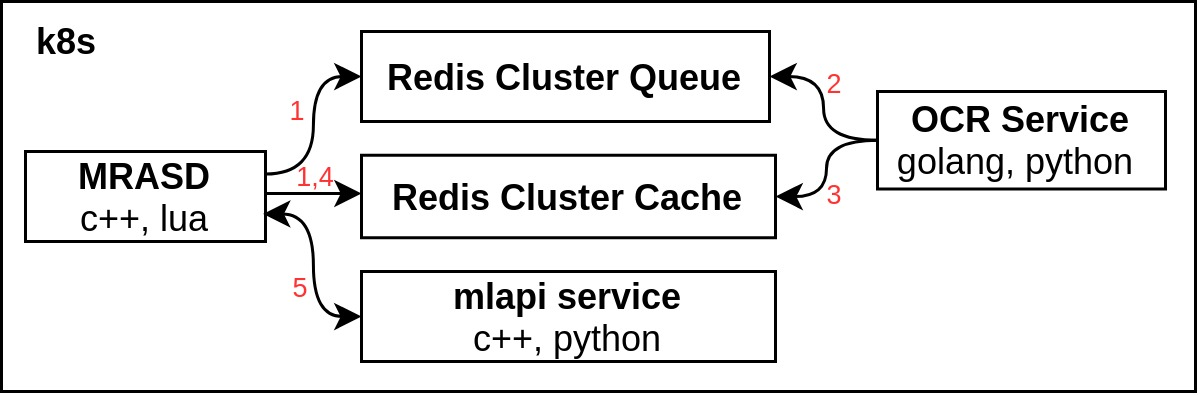
\includegraphics[width=.8\textwidth]{architecture.jpg}
\end{center}

k8s (kubernetes) --- открытое программное обеспечение для оркестровки контейнеризированных приложений и автоматизации их развертывания, масштабирования и координации в условиях кластера.

Redis --- резидентная система управления базами данных класса NoSQL с открытым исходным кодом, работающая со структурами данных типа ``ключ--значение''. Используется как для баз данных, так и для реализации кэшей, брокеров сообщений. Ориентирована на достижение максимальной производительности на атомарных операциях.

\end{frame}

%%%%%%%%%%%%%%%%%%%%%%%%%%%%%%%%%%%%%%
\begin{frame}
\frametitle{Верификация на пользователях}

\begin{center}
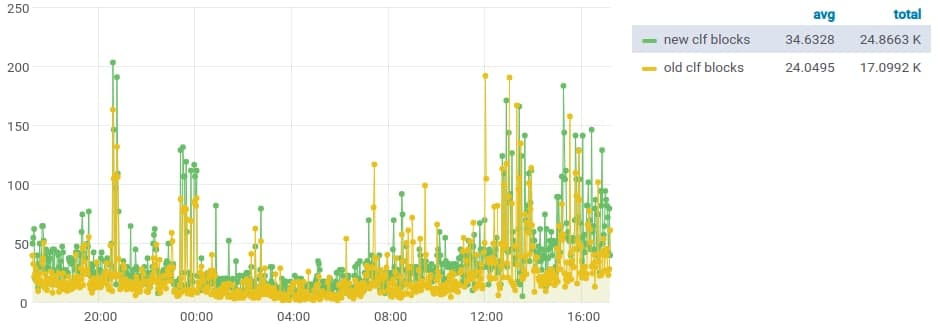
\includegraphics[width=0.9\textwidth]{old_vs_new_ps.jpg}
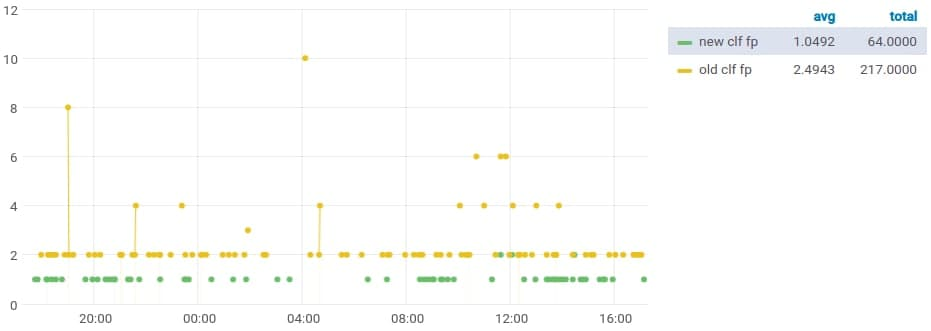
\includegraphics[width=0.9\textwidth]{old_vs_new_fp.jpg}
\end{center}

\end{frame}

%%%%%%%%%%%%%%%%%%%%%%%%%%%%%%%%%%%%%%
\begin{frame}
\frametitle{Верификация на пользователях}

\begin{center}
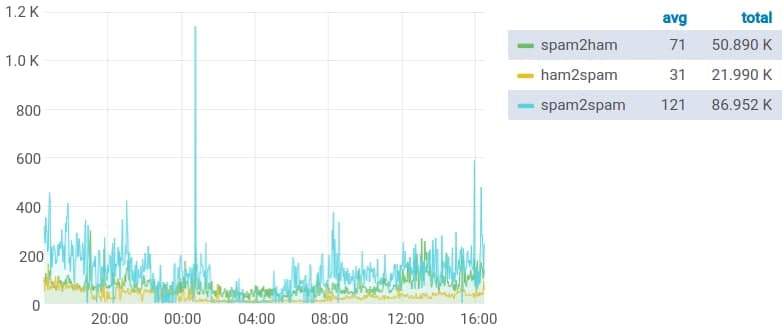
\includegraphics[width=0.75\textwidth]{old_vs_new_status.jpg}
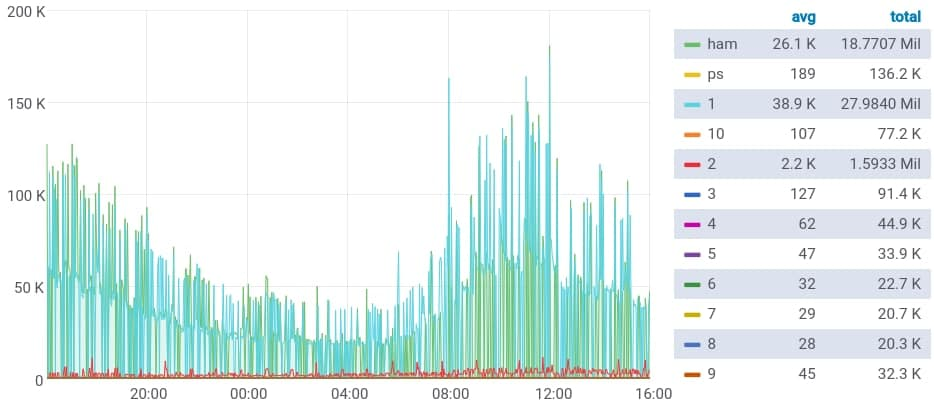
\includegraphics[width=0.75\textwidth]{dist_prob.jpg}
\end{center}

\end{frame}

%%%%%%%%%%%%%%%%%%%%%%%%%%%%%%%%%%%%%%
\begin{frame}
\frametitle{Метрики системы}

\begin{center}
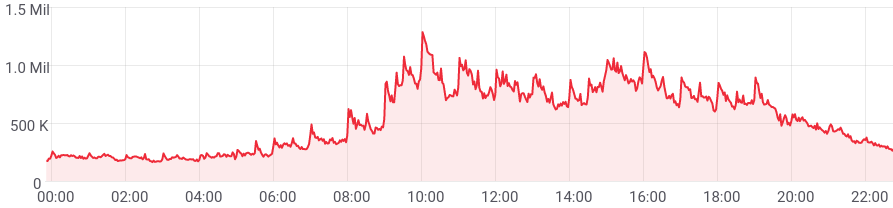
\includegraphics[width=1.0\textwidth]{processed_messages.png}
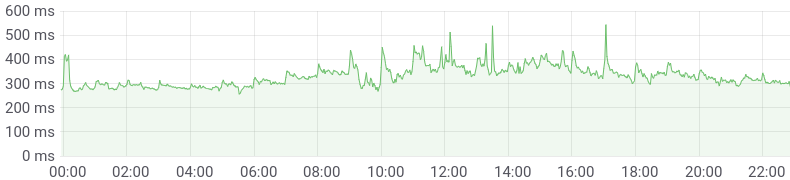
\includegraphics[width=1.0\textwidth]{timings.png}
\end{center}

\end{frame}

%%%%%%%%%%%%%%%%%%%%%%%%%%%%%%%%%%%%%%
\begin{frame}
\frametitle{Эффект от внедрения}

\begin{center}
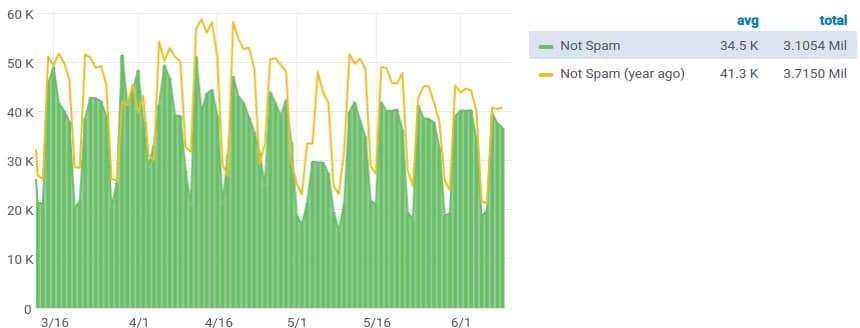
\includegraphics[width=0.8\textwidth]{is_not_spam_yeas_2_yeas.jpg}
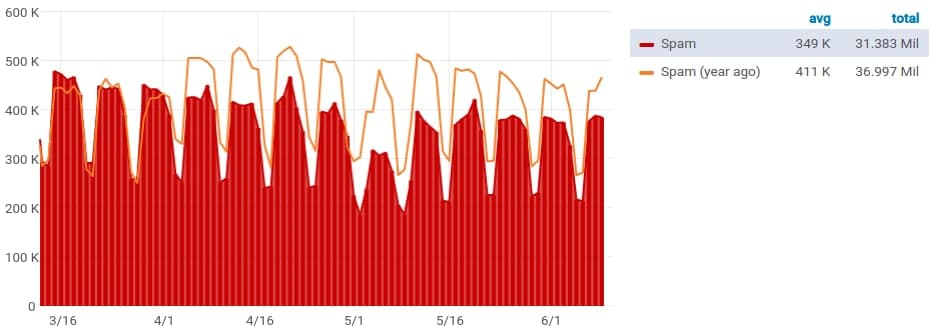
\includegraphics[width=0.8\textwidth]{is_spam_yeas_2_yeas.jpg}
\end{center}

\end{frame}

%%%%%%%%%%%%%%%%%%%%%%%%%%%%%%%%%%%%%%
\begin{frame}[fragile=singleslide]
\frametitle{Заключение}

\begin{itemize}
\item Решена задача фильтрации нежелательных данных (спам--сообщений). Анализ результатов показал, что полносвязная нейронная сеть (\verb|FCNN|) на основе алгоритма векторизации word2vec показывает лучшую точность точность классификации, по сравнению с методами классической логистической регрессии и \verb|FCNN| модели на основе алгоритма мешка слов.

\item Спроектировано и реализовано высокопризводительное отказоустойчивое приложенение, имеющее микросервисную архитектуру, которое выдерживает в среднем более $10^6$ запросов в минуту, и имеет высокое время отклика и надежность.

\item Произведен запуск приложения на реальных пользовательских продуктах Mail.ru Group, что увеличило количество блокировок спама на 10\%.
\end{itemize}

\end{frame}

%%%%%%%%%%%%%%%%%%%%%%%%%%%%%%%%%%%%%%
\begin{frame}
\frametitle{Публикации}

\begin{center}
qweqweqwe
\end{center}

\end{frame}

%%%%%%%%%%%%%%%%%%%%%%%%%%%%%%%%%%%%%%
\begin{frame}

\begin{center}
\Large\bf СПАСИБО ЗА ВНИМАНИЕ!
\end{center}

\end{frame}

\end{document}
